\documentclass[letterpaper,twocolumn,10pt]{article}

\usepackage{usenix}
\usepackage{graphicx}
\usepackage{url}
\usepackage[toc,page]{appendix}

\makeatletter
\newcommand\appendix@section[1]{%
  \refstepcounter{section}%
  \orig@section*{Appendix \@Alph\c@section: #1}%
  \addcontentsline{toc}{section}{Appendix \@Alph\c@section: #1}%
}
\let\orig@section\section
\g@addto@macro\appendix{\let\section\appendix@section}
\makeatother

% Hi Everyone, we can start with this template Cynthia gave us and go from here
% The comment feature is great for annotating text, use it!
% pdflatex should compile this just fine for now

% This file will be the main file, I just splitted the sections in different latex files, so we can modify any section in an easy and simple way. I joined all the sections in the paper using the \input{filename} command.
\begin{document}

\title{AuditBear}
\author{
{\rm David Wagner}\\
University of California at Berkeley
\and 
{\rm Cynthia Sturton}\\
University of California at Berkeley
\and 
{\rm Annie Edmundson}\\
Cornell University
\and 
{\rm Keishla Ortiz}\\
University of Puerto Rico at Arecibo
\and 
{\rm Ana Maria Quevedo}\\
Miami Dade College
\and 
{\rm Samuel Rodriguez}\\
University of Puerto Rico at Mayaguez
\and 
{\rm Patrick Baxter}\\
Clemson University
}
% Add additional authors:
% \and Author n
\maketitle

%Abstract

%Changes here (in the main paper I'll just invoke this file)
\subsection*{Abstract}
Voting audit logs produced by electronic voting systems contain information that is useful for uncovering procedural errors and election anomalies, but are currently unwieldy and difficult for election officials to use in post-election audits. In this work, we developed new methods to analyze these audit logs that includes the detection of both procedural errors and system deficiencies. We created a public web application that applies these methods to generate useful feedback on any detected issues. Election officials can use our tool to identify memory cartridges containing precinct totals that were not uploaded on election night, machines that may have experienced hardware problems during the election, and polling locations that closed late or had voters waiting in line for extended periods. We tested our analyses on data from the South Carolina 2010 elections and were able to uncover solely through the analysis of audit logs that there were 1127 votes not counted in the certified totals in Richland County, South Carolina.

%Introduction section
\section{Introduction}
Your intro goes here.

\subsection{Sub-section title}
Maybe your introduction has subsections.

%Background section
\section{Background}
\label{sec:background}
\subsection{Introduction to the iVotronic DRE}
A brief description of the iVotronic's functionality and its main
system components follows. 

\begin{itemize} 
\item \textbf{Voting terminal.} The voting terminal is a stand-alone
  touchscreen voting unit.  The terminal is equipped with an internal
  battery, which keeps the unit operational in the event of a power
  failure, and a removable compact flash card, which is used to store
  audit data and ballot images (cast vote records). Typically, each
  polling location is assigned several iVotronic machines. Also, to
  comply with the federal American with Disabilities Act, at least one
  audio terminal is placed in each precinct to assist disabled
  voters. 

\item \textbf{Personalized Electronic Ballot (PEB).} The PEB is a
  proprietary cartridge designed by ES\&S to operate the iVotronic
  terminal.  When the PEB is placed in the machine, the terminal and
  the PEB can communicate through an infrared port.  Typically,
  counties deploy two types of PEBs to the precinct: a) a master PEB
  and b) an activator PEB. Both types of PEBs have the same
  functionality, however, poll workers are trained to keep them
  separate and use them for different purposes. 
    \begin{itemize}
    \item \textbf{Master PEB.}  Poll workers use the master PEB to
      open polls on election day. When the PEB is placed in the
      terminal, the touchscreen displays the precinct's name
      programmed in the PEB so that poll workers can verify the
      polling location information and date/time registered in the
      terminal's internal clock. If the information displayed is
      correct, the poll workers open the terminal for voting. The same
      master PEB should be used to open all terminals in the polling
      location. In the same fashion, the master PEB should be used to
      close all terminals in the polling location at the end of the
      voting day. When a terminal is closed, it uploads its vote
      totals onto the PEB inserted into it. When the master PEB is
      used to close all terminals, this PEB accumulates the precinct
      totals so that they can later be uploaded and included in the
      official tally. 
    \item \textbf{Activator PEBs.}  Activator PEBs are used by  poll
      workers to activate ballots for voters. Election officials
      provide each precinct with multiple activator PEBs.  
    \end{itemize}
\end{itemize}
Internally, all PEBs at the precinct are identical. The only
difference between them is the color of the rubber band on their
exterior. Thus, a master PEB can be used to activate a voter's ballot
and an activator PEB can be used to open and close terminals. Though
as a matter of procedure and training, they should not be used this
way. If an activator PEB is used to close terminals, the precinct vote
totals may be only partially uploaded to the aggregated totals on
election night. Poll workers are trained so that they put the master
PEB, CF cards and precinct's totals tapes in a designated bag that is
transported to Election Central after polls close.  Activator PEBs
used to close terminals may be left behind and their vote data not
added to the certified count.
\begin{itemize}
\item \textbf{Removable Compact Flash (CF) card.} The CF cards are
  programmed at Election Central and installed in the back of the
  voting terminal prior to deployment at the polling location. The CF
  cards contain graphic (bitmap) files read by the voting terminal
  during the voting process. The CF cards are also used as an external
  memory device: audit log entries and ballot images are written to
  the CF card when the terminal is closed for voting. Once the polls
  close, the CF cards are removed from the back of the terminal and
  delivered to election headquarters on election night.  

\item \textbf{External printer module.} This module is connected to a
  serial port on the back of the voting terminal. The thermal printer
  produces the precinct zero tape and results tape. Poll workers are
  instructed to print the zero tape once all iVotronics of the polling
  location are opened for voting. In the same fashion, they are
  trained to print the results tape when all voting terminals are
  closed on election night. 
\end{itemize}

\subsection{iVotronic Audit}
The ES\&S voting solution produces many log files including the
Election Reporting Manager (ERM) \textquotedblleft System
Log\textquotedblright \hspace{1 mm} file, the ERM \textquotedblleft
Result Correction Log,\textquotedblright \hspace{1 mm} the ERM
\textquotedblleft Real Time Log,\textquotedblright \hspace{1 mm} the
iVotronic \textquotedblleft Ballot Image\textquotedblright \hspace{1
  mm} log and the iVotronic \textquotedblleft Event
Log.\textquotedblright \hspace{2 mm} We focus on three: the event log
(EL152.lst), ballot image file (EL155.lst), and the system log
(EL68a.lst).  The header of these log files identify the county's
name, the type and date of the election, the date the report was
generated, and the election ID. The election ID is a parameter
generated by the ES\&S election programming software to uniquely
identify each election.  
 
The event log (EL152.lst) contains audit log entries from each
iVotronic terminal used in the election.  The log  records, in
chronological order, all events that occurred on that machine during the
election. It typically begins at election headquarters, before the
election, with a \textquotedblleft clear and
test\textquotedblright \hspace{1 mm} of the terminal to delete
previous election data from the terminal's memory. It also records all
election day events, including polls open and polls closing and the
number of ballots cast.  Each event log entry includes the iVotronic's
terminal serial number, the PEB's serial number, the date and time,
the event that occurred and a description of the event. An excerpt of
an event log is given in  Appendix~\ref{app:el}. 
 
The ballot image file (EL155.lst) contains all ballot images saved by
the iVotronic terminals during the voting process. An ES\&S ballot image
is a list of all choices made for each vote cast; it is not a scanned
or photographic image. The ballot images are segregated by precinct and
terminal where the votes were cast. The ballots are saved in a random
order to protect the privacy of the voter.  An excerpt of a ballot image
file is given in Appendix~\ref{app:bi}
 
The system log listing file (EL68a.lst) chronologically tracks activity
in the election reporting database at the election headquarters. Its
entries reflect the commands executed by the operators during
pre-election testing, election night reporting, post-election testing
and canvassing. It also contains the totals accumulated in the various
precincts during election night reporting, as well as any warnings or
errors reported by the software during the tabulation process.
The system log also tracks the uploading of PEBs and CF cards to the
election reporting database. Manual adjustment of precinct totals are
also recorded in the system log file. An excerpt of a system log file is
given in Appendix~\ref{app:sl}. 

% Related Work section
\section{Related Work}
Many election technology systems provide a means of auditing elections. For example, in optical scanning systems the cast ballots form a paper record of the votes cast.  On the other hand, paperless DRE machines do not provide this type of paper trail. Some DRE systems provide a Voter Verified Paper Audit Trail (VVPAT), which stores a hard copy version of each ballot cast.  A third type of audit trail, which is produced by all DREs, are the event logs stored electronically on each DRE.  In this section we discuss related work on the analysis of audit logs for post-election auditing. 

Two recent studies used event logs from the iVotronic voting system to audit elections~\cite{Buell2011,Sandler2007}. The authors of the first study~\cite{Buell2011} performed an audit of the same South Carolina elections that we analyzed. Using these audit logs, they discovered votes not included in the certified counts and problems with the audit data. They crosschecked the event log, the ballot image file, and the system log to identify unsupported votes and missing audit data.  By consulting additional audit materials, such as the printed results tapes, the authors were able to offer possible reasons and explanations as to why the problems occurred. Our work takes a slightly different approach.  We focus on developing a variety of methods to analyze the data; in addition, we automate these analyses for use by election officials.  While our tool did discover and report similar problems, we simply report what was wrong, but can not provide a possible explanation for the cause of the error as we didn't have access to printed results tapes. 

The authors of the second study~\cite{Sandler2007} provided an analysis of vote tallies using the protected count of votes on each machine and comparing this to the printed results tapes. Their report also finds date/time stamps that were most likely inaccurate.  With further investigation, they concluded that the machine hardware clock was incorrect. Our research provides analyses to identify similar problems, but in a way that could be automated. 

There has also been research on using the audit logs to analyze election-day procedure and activity. For example, one recent publication showed how event logs could be used to determine if a machine acted \textquotedblleft normally\textquotedblright on election day~\cite{Antonyan2009}. The authors of this research studied the event logs of the AccuVote Optical Scanning system and used those logs to build a finite state machine that models the sequences of events that a well-behaved machine might produce. This type of analysis would be useful to provide for the iVotronic systems that we studied. However, the AccuVote machines have considerably fewer possible event types than the iVotronics so the analysis would become considerably more complex. 

A common problem on election day, which we try to identify in our analysis, is the occurrence of long lines. Many studies have researched ways to mitigate long lines at polling locations ~\cite{Allen2006,Dow2007,Spencer2010,Wilson2008,Edel2010}.  One such study has simulated the flow of voters through the voting process~\cite{Edel2010}. The authors use this simulation to determine the optimal number of voters per voting machine, and correspondingly, the appropriate number of voting machines per polling location based on the number of registered voters at that particular location. Their work is predictive: the authors make some assumptions, such as the average time it takes to vote and when peak voting hours will occur, and use those as a basis for predicting where long lines are likely to occur. Our analysis is descriptive: given the audit logs from election day, we infer the average time it took to vote and use that information to determine whether a particular polling location experienced long lines or not. The two methods are complementary. Predictive models can be used to prevent long lines, while descriptive models can be used to check and refine the prediction algorithms. 

Voter Verified Paper Audit Trails (VVPATs) are a different type of audit log. Unlike the audit logs we used in our analyses, VVPATs are viewed and verified by the voter and are more suited to audits concerning a DRE incorrectly capturing a voter\textquoteright s intent. Our work is more concerned with identifying cases of cast votes not being included in the final count, or issues at the polling place that might prevent the voter from casting their vote in the first place. With VVPATs, as long as a certain percentage of voters do check their paper ballot~\cite{Hall2006}, the voting machine need not be assumed correct, whereas our analyses do make this assumption.

%Conclusion
\section{Conclusion}
In this study we developed a tool to analyze audit data from DRE voting machines. Our web based application, accessible to anyone, performs a variety of analyses on the audit data to detect procedural errors and system deficiencies. We replicated a previous study conducted using iVotronic audit logs collected in South Carolina after the 2010 Primary and General elections~\cite{Buell2011}. The aforementioned paper identified media devices containing votes that were not included in the certified totals. In addition, our tool can identify terminals that were not closed and their votes not uploaded to the cumulative count. This information can be very useful during the canvass process as election officials can locate the missing terminals, close them and add their votes to the election totals. 

Having performed analyses with the iVotronic logs from South Carolina, we also report statistics on polling location procedures. These statistics include: polling locations that closed late or may have experienced long lines of voters, precincts which did not report the zero tape and polling locations which used the wrong device to activate ballots on election day. Our tool can also report statistics concerning possible DRE hardware problems such as calibration issues, low battery and incorrect date and time settings. With this information election officials can improve their poll worker training or schedule voting machine repairs as needed.

%This point is going to need more work.  I'm thinking if we expand on it we might want something about Wagner's work in either our introduction or related works section.
Dr. Wagner's commissioned report ,  "Voting Systems Audit Log Study" extensively documents and evaluates many different types of audit logs produced by six different voting systems.  In the findings there were no machines that provided tools, support, or generated summary reports for analyzing audit logs.~\cite{Wagner2010}. While, the authors are very familiar with the strengths and weaknesses of the iVotronic's audit logs we would direct anyone interested in the future design of audit logs to this report.  Fully documenting the strengths and weaknesses of the iVotronic audit systems is outside the scope of this project. Our website is only the first step in creating a process for automated election auditing.  We hope that future third-party audit log  tools can build on some of this previous work to create a useful and robust solution for deriving meaningful audits directly from the logs.

We recommend that election administrators conduct routine reviews of the audit logs generated by the voting machines as they are ground truth for election disputes. By automating our analyses and making it as simple as uploading the iVotronic audit logs to a website, we believe our tool can standardize the post-election audits performed by the iVotronic system users. Our website can quickly provide intelligent feedback to election officials during the canvassing process and serve to influence future audit procedures. 

%Acknowledgements section
\section{Acknowledgments}
We thank David Wagner and Cynthia Sturton for their support and contribution.  Special thanks to Dr. Kristen Gates, National Science Foundation and the TRUST program staff.

%This tells latex to use our .bib file
\bibliographystyle{plain}
{\footnotesize
\bibliography{paper}}

%Appendix section
\clearpage
\onecolumn
\begin{center}
\appendix
\section{Event Log File}\label{app:el} 
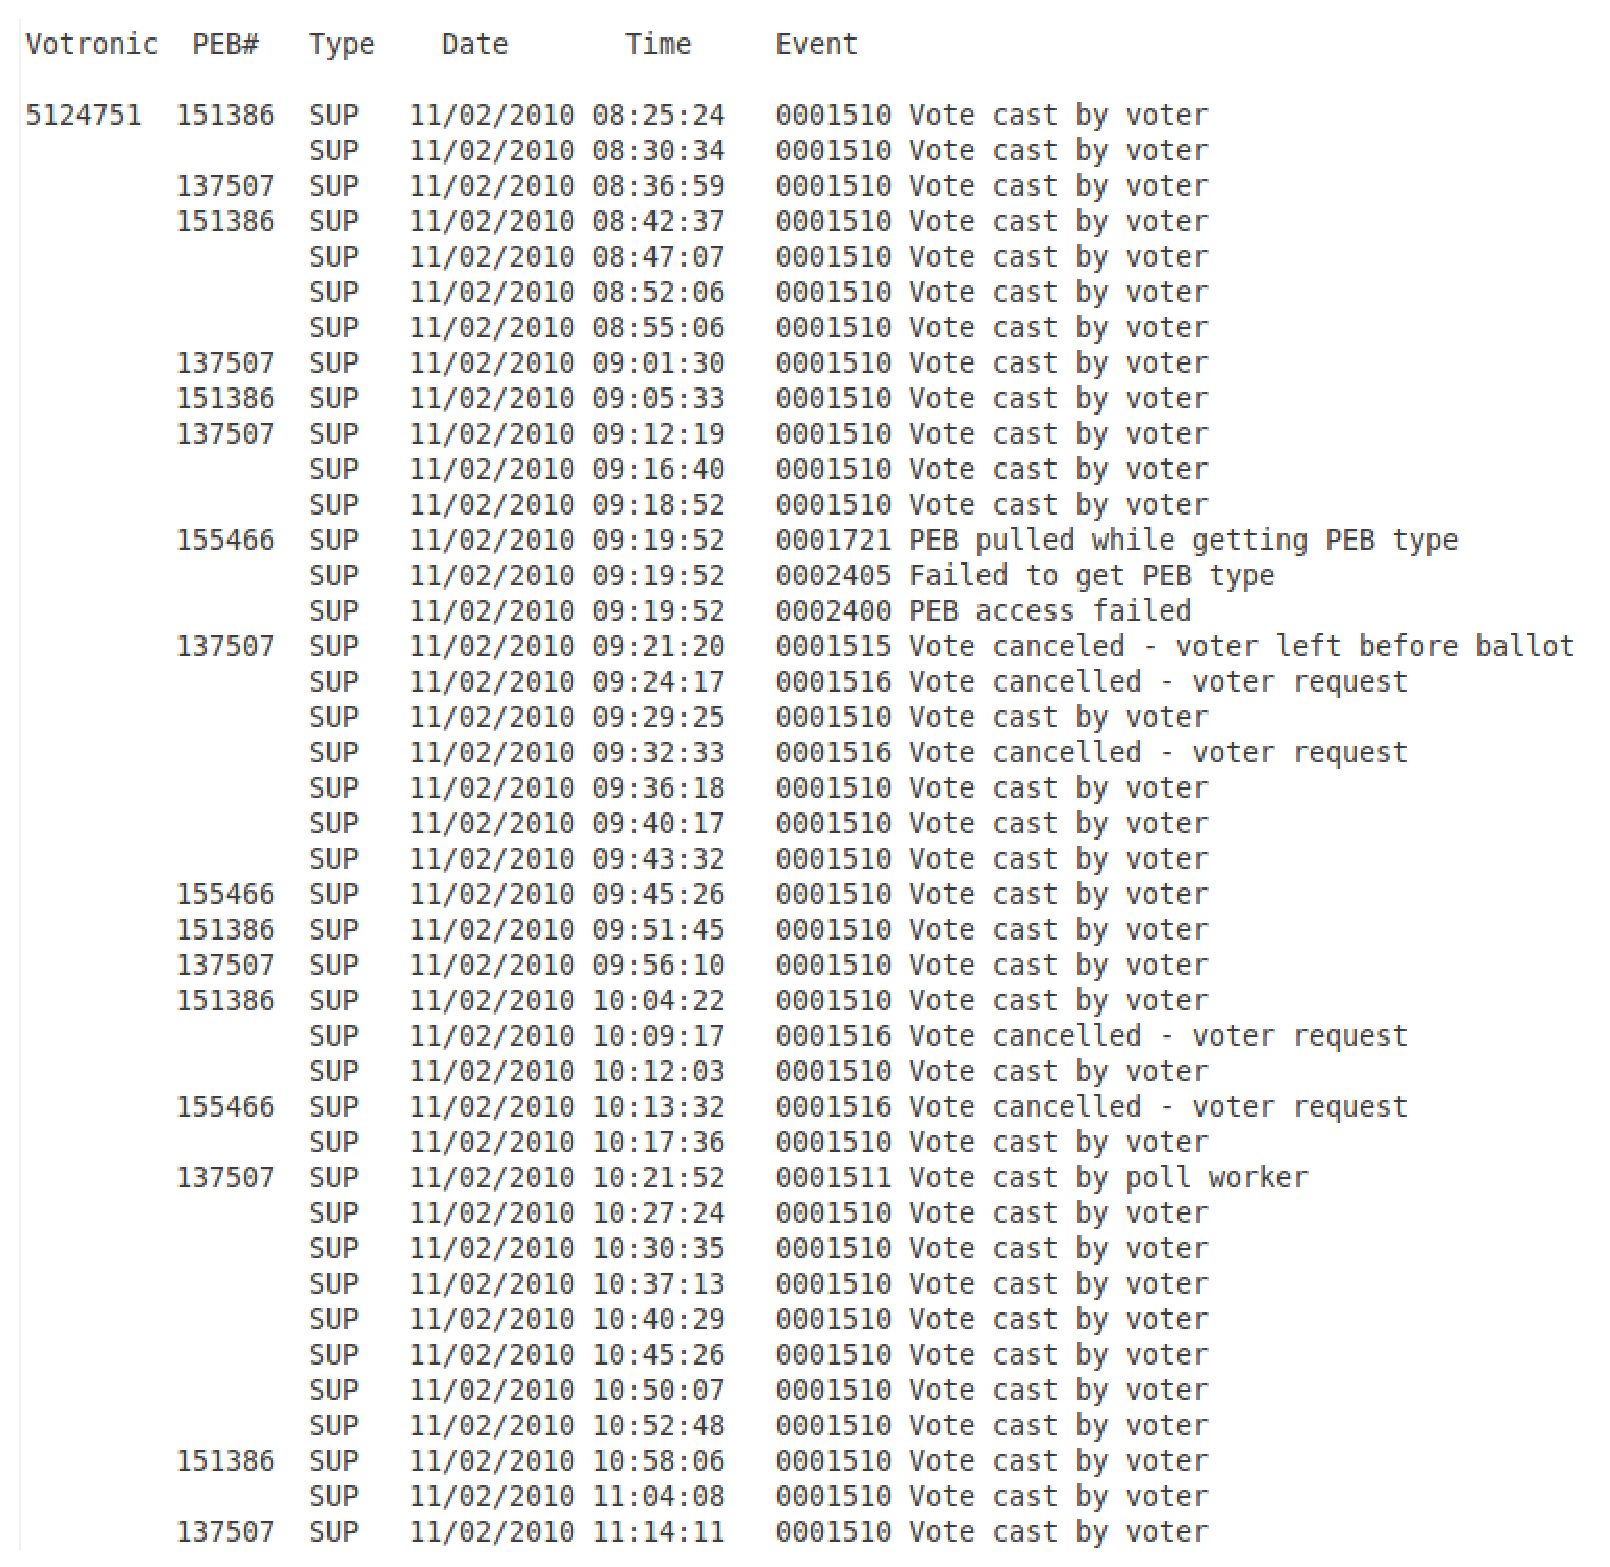
\includegraphics[width=0.8\textwidth]{eventLog}
%~\ref{app:el}

\clearpage
\section{Ballot Image File}\label{app:bi}
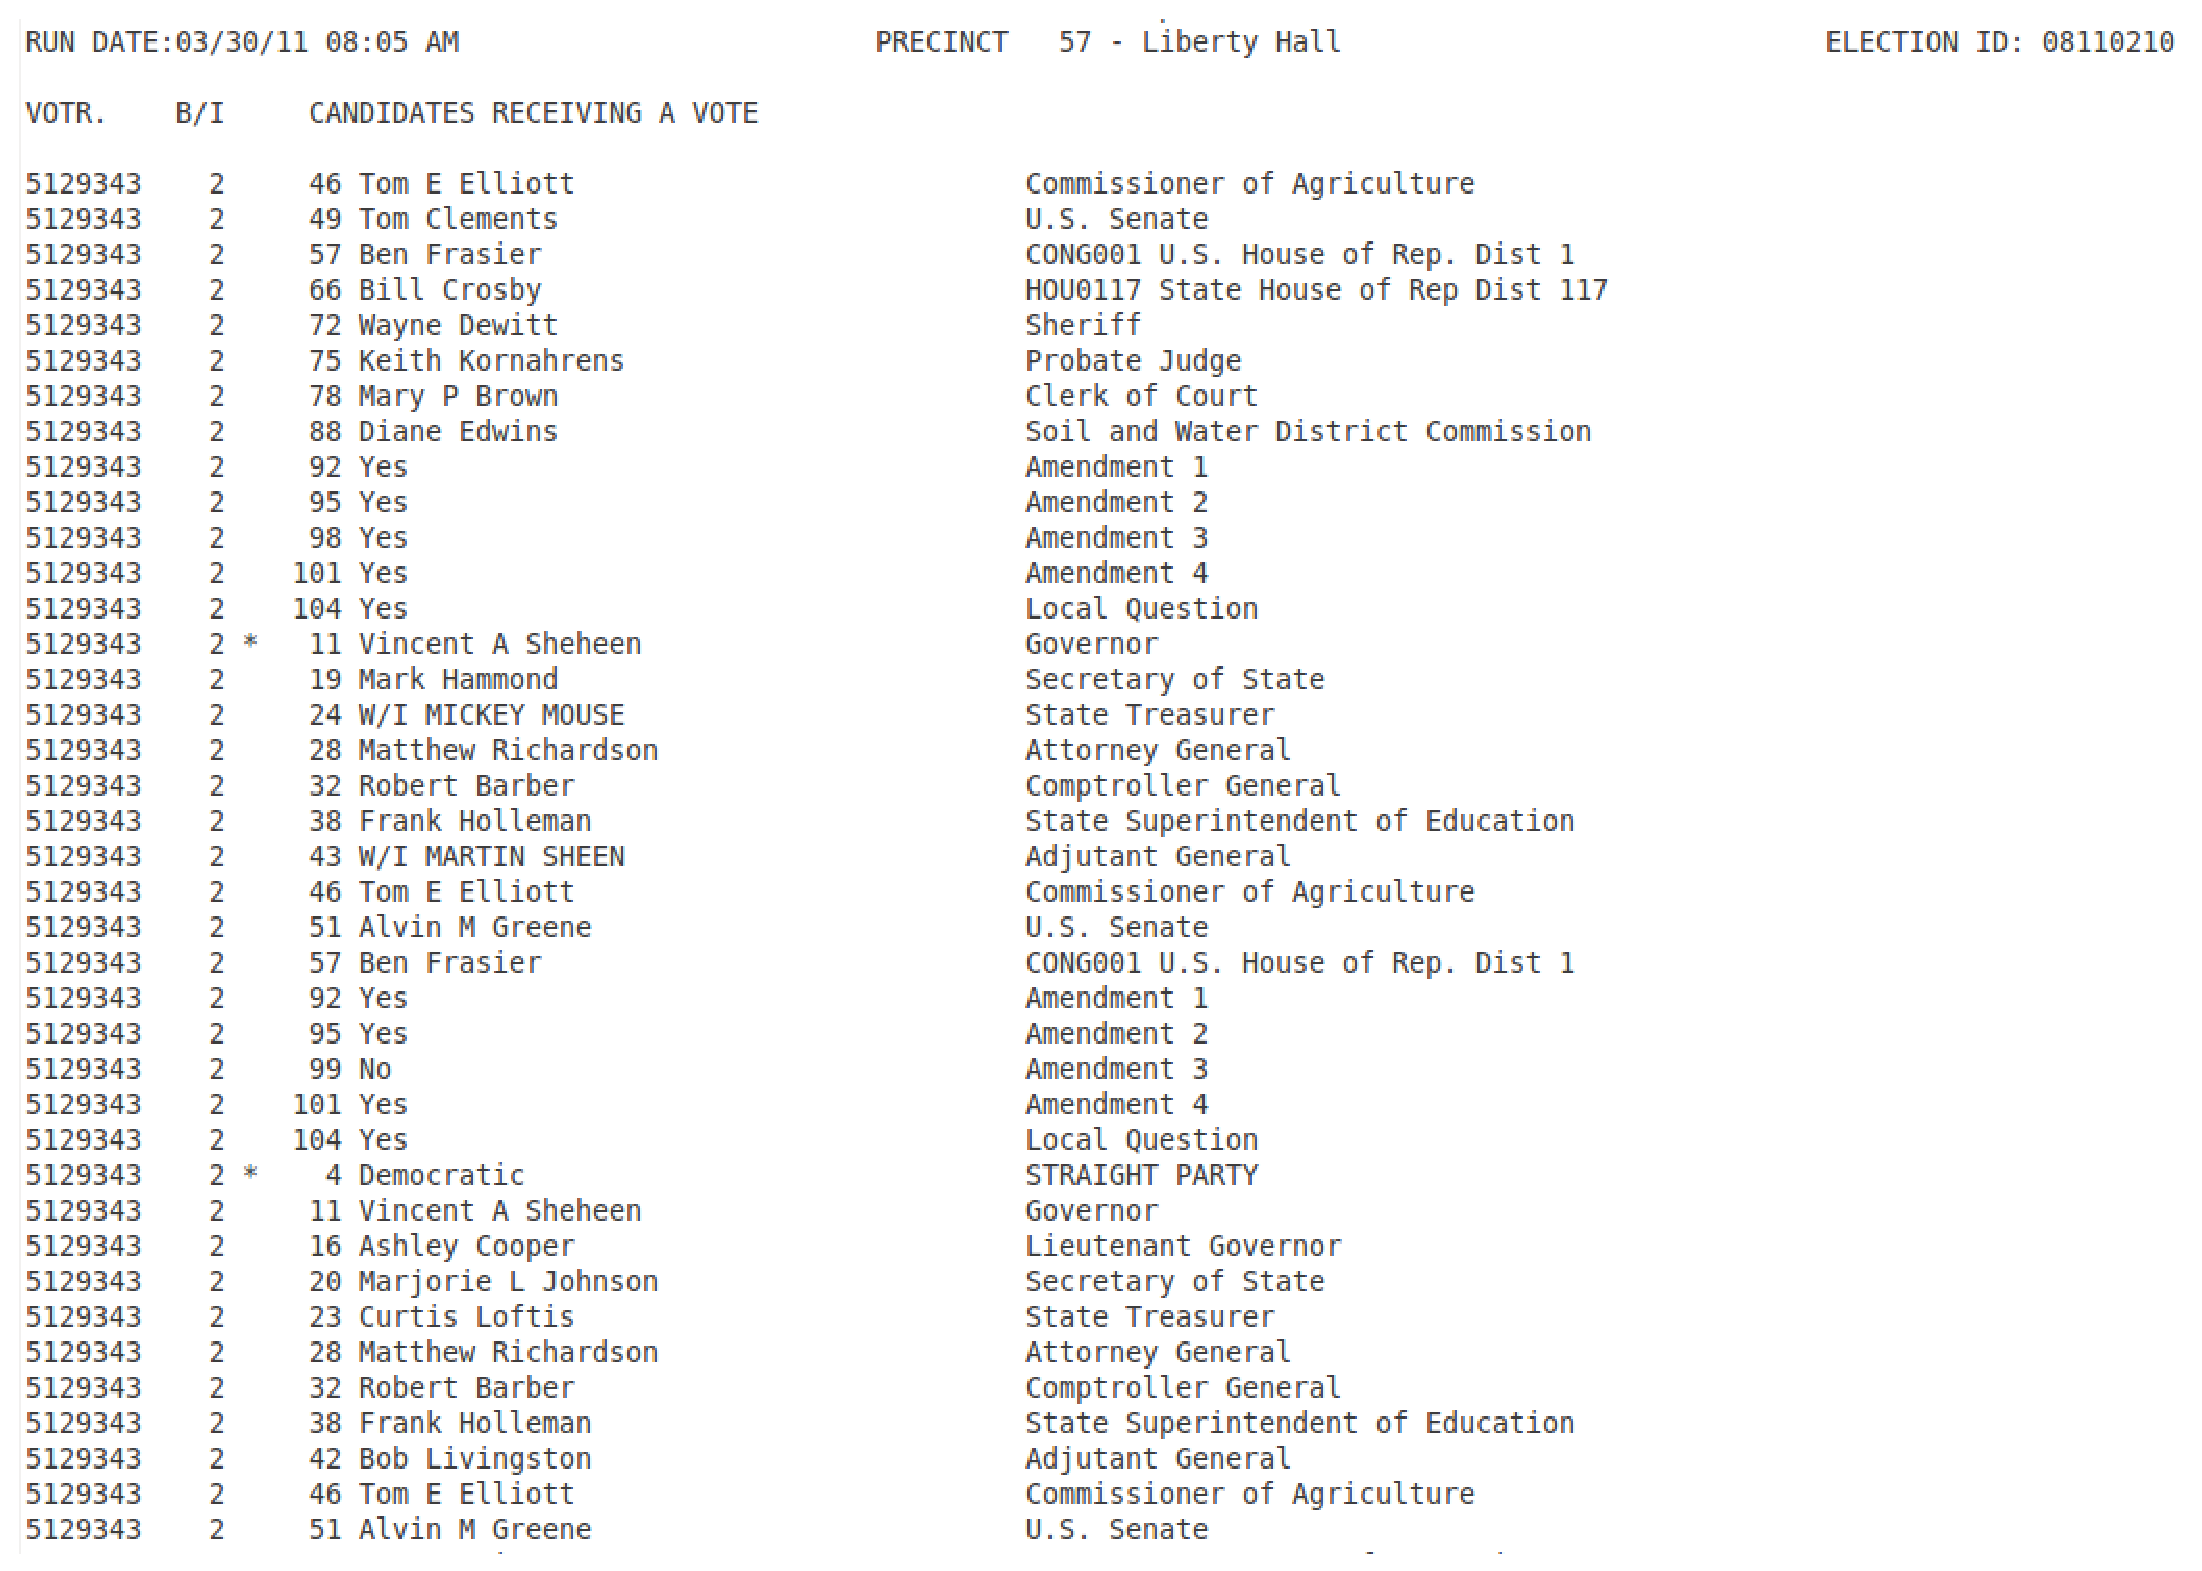
\includegraphics[width=0.9\textwidth]{ballot}
%This is app~\ref{app:bi}

\clearpage
\section{System Log File}\label{app:sl}
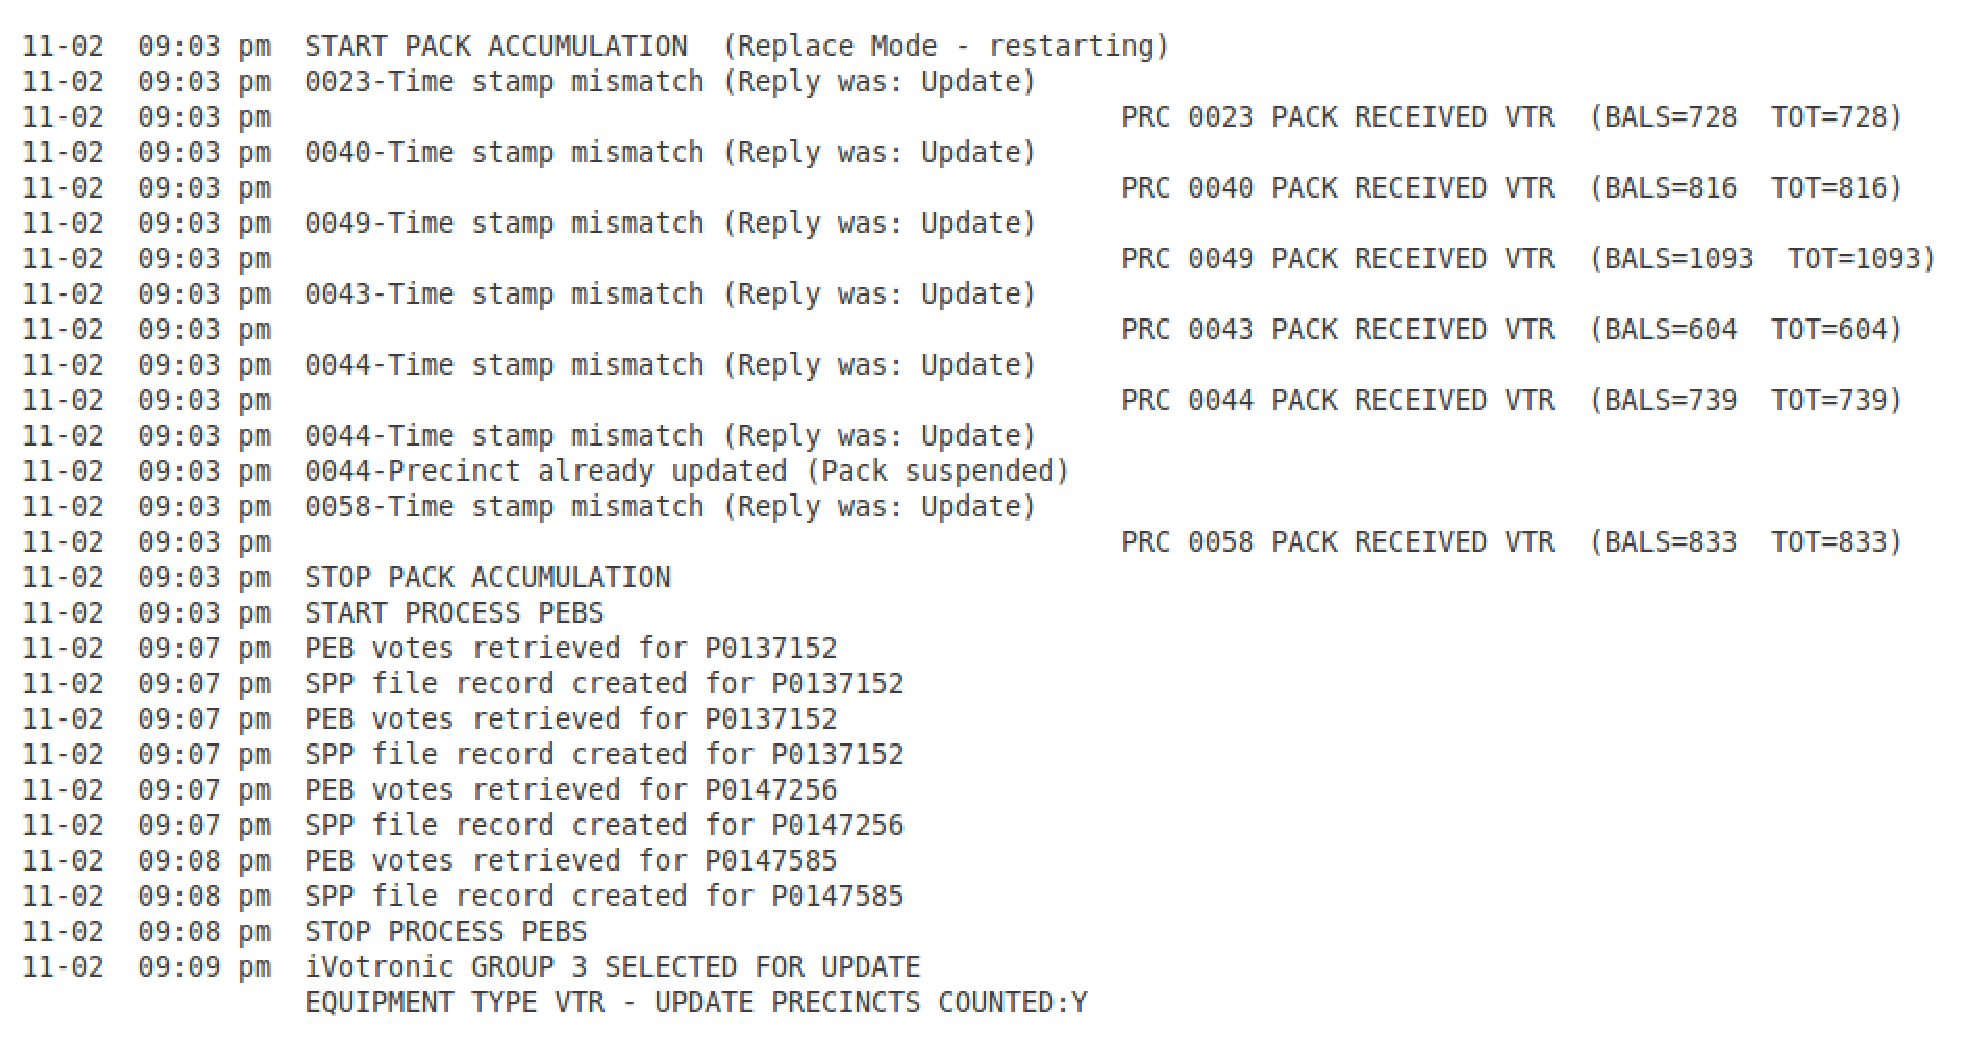
\includegraphics[width=0.9\textwidth]{system}
%This is app~\ref{app:sl}
\end{center}


\end{document}
